\documentclass[aspectratio=169, table]{beamer}
\usepackage[utf8]{inputenc}
\usepackage{listings} 
\usepackage[strings]{underscore}
\usepackage{caption}
\usepackage{float}

\usepackage{tikz}
\usetikzlibrary{positioning, trees}



\renewcommand{\lstlistingname}{} 

\makeatletter
\def\input@path{{../../themes/Pradita}}
\makeatother

\usetheme{Pradita}

\subtitle{IF120203-Programming Fundamentals}

\title{Chapter-08:\\\LARGE{Pemrograman Berorientasi Objek\\}
\vspace{10pt}}
\date[Serial]{\scriptsize {PRU/SPMI/FR-BM-18/0222}}
\author[Pradita]{\small{\textbf{Alfa Yohannis}}}


% Define Python language style for listings
\lstdefinestyle{PythonStyle}{
    language=Python,
    basicstyle=\ttfamily\footnotesize,
    keywordstyle=\color{blue}\bfseries,
    commentstyle=\color{gray}\itshape,
    stringstyle=\color{red},
    showstringspaces=false,
    breaklines=true,
    frame=lines,
    numbers=left,
    numberstyle=\tiny\color{gray},
    backgroundcolor=\color{lightgray!10},
    tabsize=2,
    captionpos=b
}

\lstdefinelanguage{bash} {
	keywords={},
	basicstyle=\ttfamily\small,
	keywordstyle=\color{blue}\bfseries,
	ndkeywords={iex},
	ndkeywordstyle=\color{purple}\bfseries,
	sensitive=true,
	commentstyle=\color{gray},
	stringstyle=\color{red},
	numbers=left,
	numberstyle=\tiny\color{gray},
	breaklines=true,
	frame=lines,
	backgroundcolor=\color{lightgray!10},
	tabsize=2,
	comment=[l]{\#},
	morecomment=[s]{/*}{*/},
	commentstyle=\color{gray}\ttfamily,
	stringstyle=\color{purple}\ttfamily,
	showstringspaces=false,
	captionpos=b
}

\begin{document}

\frame{\titlepage}

% Add table of contents slide
\begin{frame}[fragile]{Contents}
\vspace{15pt}
\begin{columns}[t]
\begin{column}{.4\textwidth}
\tableofcontents[sections={1-4}]
\end{column}
\begin{column}{.6\textwidth}
\tableofcontents[sections={5-7}]
\end{column}
\end{columns}
\end{frame}


\section{Pengenalan OOP}

\begin{frame}[fragile]{Pengenalan OOP}
\vspace{20pt}
\begin{itemize}
    \item Pemrograman Berorientasi Objek (OOP) berfokus pada pembuatan \emph{objek} yang merepresentasikan entitas dunia nyata.
    \item Setiap objek memiliki \emph{atribut} (data) dan \emph{metode} (perilaku).
    \item Berbeda dengan pendekatan prosedural yang berorientasi pada fungsi.
    \item OOP menekankan struktur dan hubungan antar objek.
    \item Tujuan utamanya adalah membuat kode yang mudah dipelihara, diperluas, dan digunakan kembali.
\end{itemize}
\end{frame}

\begin{frame}[fragile]{Konsep Utama OOP}
\vspace{20pt}
\begin{itemize}
    \item \textbf{Kelas}: cetak biru untuk membuat objek.  
    \item \textbf{Objek}: instance nyata dari kelas.  
    \item \textbf{Atribut}: data yang dimiliki objek.  
    \item \textbf{Metode}: perilaku atau fungsi dalam kelas.  
    \item \textbf{Pewarisan}: mewarisi sifat kelas lain.  
    \item \textbf{Polimorfisme}: objek berbeda merespons cara yang sama dengan hasil berbeda.
\end{itemize}
\end{frame}

\begin{frame}[fragile]{Contoh Pendekatan OOP}
\vspace{20pt}
\begin{lstlisting}[style=PythonStyle]
class Orang:
    def __init__(self, nama, umur):
        self.nama = nama
        self.umur = umur

    def sapa(self):
        print(f"Halo {self.nama}, umur kamu {self.umur} tahun.")

o1 = Orang("Rani", 21)
o1.sapa()
\end{lstlisting}
OOP menyatukan data dan perilaku dalam satu kesatuan logis, yaitu \textbf{objek}.
\end{frame}

\section{Kelas dan Objek}

\begin{frame}[fragile]{Konsep Kelas dan Objek}
\vspace{20pt}
\begin{itemize}
    \item \textbf{Kelas} adalah cetak biru/definisi sebuah objek.
    \item \textbf{Objek} adalah wujud nyata dari definisi kelas.
    \item Kelas menetapkan atribut (data) dan metode (perilaku).
    \item Semua objek dari kelas yang sama berbagi struktur/perilaku, namun datanya dapat berbeda.
    \item Tujuan: model yang jelas, kode mudah dipelihara dan diperluas.
\end{itemize}
\end{frame}

\begin{frame}[fragile]{Kelas sebagai Definisi Objek (Kode)}
\vspace{20pt}
\begin{columns}[T]
\begin{column}{0.55\textwidth}
\begin{lstlisting}[style=PythonStyle]
# Definisi kelas Mahasiswa
class Mahasiswa:
    def __init__(self, nama, nim):
        self.nama = nama
        self.nim = nim

# Objek adalah wujud nyata dari definisi di atas
m1 = Mahasiswa("Rani", "A11.2024.0001")
m2 = Mahasiswa("Dani", "A11.2024.0002")

print(m1.nama)  # Rani
print(m2.nama)  # Dani
\end{lstlisting}
\end{column}

\begin{column}{0.4\textwidth}
\textbf{Penjelasan:}
\begin{itemize}
    \item \textbf{Kelas} mendefinisikan struktur dan perilaku suatu objek.
    \item \textbf{Objek} adalah realisasi nyata dari kelas tersebut.
    \item Setiap objek memiliki data sendiri, tetapi mengikuti cetak biru yang sama.
    \item Contoh: \texttt{m1} dan \texttt{m2} adalah dua objek dari kelas \texttt{Mahasiswa}.
\end{itemize}
\end{column}
\end{columns}
\end{frame}


\begin{frame}[fragile]{Membuat Kelas dan Objek (Kode)}
\vspace{20pt}
\begin{lstlisting}[style=PythonStyle]
class Mobil:
    def __init__(self, merek, warna):
        self.merek = merek
        self.warna = warna

    def info(self):
        print(f"Mobil {self.merek} berwarna {self.warna}")

# Membuat beberapa objek dari satu definisi kelas
mobil1 = Mobil("Toyota", "Merah")
mobil2 = Mobil("Honda", "Putih")

mobil1.info()
mobil2.info()
\end{lstlisting}
\end{frame}

\begin{frame}[fragile]{Relasi Kelas–Objek (Skema)}
\vspace{20pt}
\begin{columns}[T]
\begin{column}{0.55\textwidth}
\begin{center}
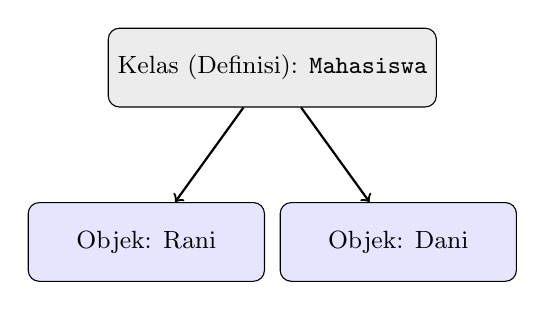
\begin{tikzpicture}[node distance=2.8cm, every node/.style={font=\small}]
\node (class) [draw, rectangle, rounded corners, fill=gray!15,
minimum width=4cm, minimum height=1cm]
{Kelas (Definisi): \texttt{Mahasiswa}};
\node (obj1) [below=1.2cm of class, xshift=-1.6cm, draw, rectangle,
rounded corners, fill=blue!10, minimum width=3cm, minimum height=1cm]
{Objek: Rani};
\node (obj2) [below=1.2cm of class, xshift=1.6cm, draw, rectangle,
rounded corners, fill=blue!10, minimum width=3cm, minimum height=1cm]
{Objek: Dani};
\draw[->, thick] (class) -- (obj1);
\draw[->, thick] (class) -- (obj2);
\end{tikzpicture}
\end{center}
\end{column}

\begin{column}{0.4\textwidth}
\textbf{Penjelasan:}
\begin{itemize}
    \item \textbf{Kelas} mendefinisikan struktur dan perilaku objek.
    \item \textbf{Objek} adalah realisasi/wujud dari kelas (\textbf{konsep/definisi}), dengan data masing-masing.
    \item \texttt{Rani} dan \texttt{Dani} merupakan contoh objek dari kelas \texttt{Mahasiswa}.
\end{itemize}
\end{column}
\end{columns}
\end{frame}



\section{Atribut dan Metode}

\begin{frame}[fragile]{Konsep Atribut dan Metode}
\vspace{20pt}
\begin{itemize}
    \item \textbf{Atribut} menyimpan data atau keadaan objek.
    \item \textbf{Metode} mendefinisikan perilaku atau aksi objek.
    \item Atribut menunjukkan \emph{apa yang dimiliki} oleh objek.
    \item Metode menunjukkan \emph{apa yang dapat dilakukan} oleh objek.
    \item Dalam Python, atribut dibedakan menjadi:
    \begin{itemize}
        \item \textbf{Atribut Instans} — milik masing-masing objek.
        \item \textbf{Atribut Kelas} — dimiliki bersama oleh semua objek.
    \end{itemize}
\end{itemize}
\end{frame}

\begin{frame}[fragile]{Atribut Instans dan Kelas (Contoh 1)}
\vspace{20pt}
\begin{lstlisting}[style=PythonStyle]
class Mahasiswa:
    def __init__(self, nama, nim):
        self.nama = nama      # atribut instans
        self.nim = nim        # atribut instans

m1 = Mahasiswa("Rani", "A11.2024.0001")
m2 = Mahasiswa("Dani", "A11.2024.0002")

print(m1.nama)  # Rani
print(m2.nama)  # Dani
\end{lstlisting}
Atribut instans berbeda untuk setiap objek dan disimpan di dalam \texttt{self}.
\end{frame}

\begin{frame}[fragile]{Atribut Kelas dan Perubahannya (Contoh 2)}
\vspace{20pt}
\begin{columns}[T]
\begin{column}{0.55\textwidth}
\begin{lstlisting}[style=PythonStyle]
class Mahasiswa:
    universitas = "Pradita University"  # atribut kelas

    def __init__(self, nama, nim):
        self.nama = nama
        self.nim = nim

m1 = Mahasiswa("Rani", "A11.2024.0001")
m2 = Mahasiswa("Dani", "A11.2024.0002")

print(m1.universitas)  
# Pradita University
print(m2.universitas)  
# Pradita University
\end{lstlisting}
\end{column}

\begin{column}{0.4\textwidth}
\begin{lstlisting}[style=PythonStyle]
Mahasiswa.universitas = "Universitas Python"

print(m1.universitas)  
# Universitas Python
print(m2.universitas)  
# Universitas Python
\end{lstlisting}

\textit{Atribut kelas digunakan bersama oleh semua objek 
dan berubah serentak ketika nilainya diperbarui.}
\end{column}
\end{columns}
\end{frame}


\section{Metode dan \texttt{self}}

\begin{frame}[fragile]{Konsep Metode dan self}
\vspace{20pt}
\begin{itemize}
    \item \textbf{Metode} adalah fungsi di dalam kelas yang menggambarkan perilaku objek.
    \item Setiap metode memiliki parameter pertama bernama \texttt{self}.
    \item \texttt{self} mengacu pada objek yang memanggil metode tersebut.
    \item Dengan \texttt{self}, metode dapat mengakses dan mengubah atribut milik objek.
    \item Pemanggilan seperti \texttt{obj.metode()} secara otomatis meneruskan objek \texttt{obj} ke parameter \texttt{self}.
\end{itemize}
\end{frame}

\begin{frame}[fragile]{Contoh Metode dengan self}
\vspace{20pt}
\begin{lstlisting}[style=PythonStyle]
class Mahasiswa:
    def __init__(self, nama, nim):
        self.nama = nama
        self.nim = nim

    def sapa(self):
        print(f"Halo, saya {self.nama} ({self.nim})")

m1 = Mahasiswa("Rani", "A11.2024.0001")
m2 = Mahasiswa("Dani", "A11.2024.0002")

m1.sapa()
m2.sapa()
\end{lstlisting}
Metode \texttt{sapa()} menggunakan \texttt{self} untuk menampilkan data milik objek pemanggil.
\end{frame}

\begin{frame}[fragile]{Metode yang Mengubah Keadaan Objek}
\vspace{10pt}
\begin{lstlisting}[style=PythonStyle]
class Mobil:
    def __init__(self, merek, kecepatan=0):
        self.merek = merek
        self.kecepatan = kecepatan

    def tambah_kecepatan(self, delta):
        self.kecepatan += delta

    def info(self):
        print(f"{self.merek} melaju {self.kecepatan} km/jam")

mobil1 = Mobil("Toyota")
mobil1.tambah_kecepatan(50)
mobil1.info()
\end{lstlisting}
Metode \texttt{tambah\_kecepatan()} mengubah atribut, sedangkan \texttt{info()} menampilkan hasilnya.
\end{frame}

\begin{frame}[fragile]{Ringkasan: Atribut, Metode, dan self}
\vspace{10pt}
\begin{center}
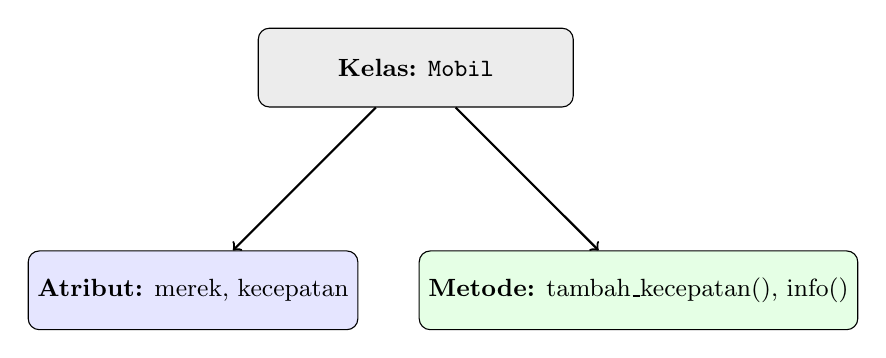
\begin{tikzpicture}[node distance=4cm, every node/.style={font=\small}]
\node (class) [draw, rectangle, rounded corners, fill=gray!15, 
minimum width=4cm, minimum height=1cm] 
{\textbf{Kelas:} \texttt{Mobil}};
\node (attr) [below left of=class, draw, rectangle, rounded corners, 
fill=blue!10, minimum width=3cm, minimum height=1cm] 
{\textbf{Atribut:} merek, kecepatan};
\node (method) [below right of=class, draw, rectangle, rounded corners, 
fill=green!10, minimum width=3cm, minimum height=1cm] 
{\textbf{Metode:} tambah\_kecepatan(), info()};
\draw[->, thick] (class) -- (attr);
\draw[->, thick] (class) -- (method);
\end{tikzpicture}
\end{center}

\subsection*{Ringkasan}
\begin{itemize}
    \item \textbf{Atribut} menyimpan data atau keadaan objek.
    \item \textbf{Metode} mendefinisikan perilaku objek.
    \item \texttt{self} digunakan untuk mengakses atribut dan metode milik objek itu sendiri.
    \item Atribut kelas dimiliki bersama, sedangkan atribut instans spesifik untuk tiap objek.
\end{itemize}
\end{frame}

\section{Pewarisan (Inheritance)}

\begin{frame}[fragile]{Konsep Pewarisan (Inheritance)}
\vspace{20pt}
\begin{itemize}
    \item \textbf{Pewarisan} memungkinkan kelas baru mewarisi atribut dan metode dari kelas lain.
    \item Kelas induk disebut \textbf{superclass}, dan kelas turunan disebut \textbf{subclass}.
    \item Subclass dapat:
    \begin{itemize}
        \item Menggunakan atribut dan metode kelas induk.
        \item Menambahkan fitur baru.
        \item Menimpa (\emph{override}) perilaku lama.
    \end{itemize}
\end{itemize}
\begin{center}
\textit{Tujuan utama: memanfaatkan kembali kode dan membangun hierarki kelas yang logis.}
\end{center}
\end{frame}

\begin{frame}[fragile]{Contoh Pewarisan Dasar}
\vspace{20pt}
\begin{columns}[T]
\begin{column}{0.65\textwidth}
\begin{lstlisting}[style=PythonStyle]
# Kelas induk
class Kendaraan:
    def __init__(self, merek):
        self.merek = merek

    def info(self):
        print(f"Kendaraan merek {self.merek}")

# Kelas turunan
class Mobil(Kendaraan):
    def __init__(self, merek, jumlah_pintu):
        self.merek = merek
        self.jumlah_pintu = jumlah_pintu

    def info(self):
        print(f"Mobil {self.merek} dengan {self.jumlah_pintu} pintu")
\end{lstlisting}
\end{column}

\begin{column}{0.3\textwidth}
\begin{lstlisting}[style=PythonStyle]
k1 = Kendaraan("Yamaha")
m1 = Mobil("Toyota", 4)

k1.info()
m1.info()
\end{lstlisting}

\textit{Kelas \texttt{Mobil} menambah atribut baru 
dan menimpa metode \texttt{info()} dari kelas induk.}
\end{column}
\end{columns}
\end{frame}


\begin{frame}[fragile]{Diagram Relasi Kelas Induk dan Turunan}
\vspace{20pt}
\begin{center}
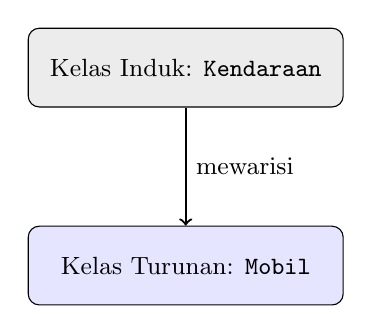
\begin{tikzpicture}[node distance=2.8cm, every node/.style={font=\small}]
\node (super) [draw, rectangle, rounded corners, fill=gray!15, 
minimum width=4cm, minimum height=1cm] 
{Kelas Induk: \texttt{Kendaraan}};
\node (child) [below=1.5cm of super, draw, rectangle, rounded corners, 
fill=blue!10, minimum width=4cm, minimum height=1cm] 
{Kelas Turunan: \texttt{Mobil}};
\draw[->, thick] (super) -- (child) node[midway, right] {mewarisi};
\end{tikzpicture}
\end{center}
\begin{itemize}
    \item Pewarisan menghindari duplikasi kode.
    \item Memudahkan perluasan fungsi.
    \item Menyusun struktur hierarki antar kelas.
\end{itemize}
\end{frame}

\begin{frame}[fragile]{Hierarki Pewarisan Bertingkat}
\vspace{20pt}
\begin{columns}[t]
\begin{column}{0.55\textwidth}
\begin{lstlisting}[style=PythonStyle]
class Kendaraan:
    def bergerak(self):
        print("Kendaraan bergerak")

class Mobil(Kendaraan):
    def bergerak(self):
        print("Mobil melaju di jalan")

class MobilBalap(Mobil):
    def bergerak(self):
        print("Mobil balap melaju sangat cepat!")
\end{lstlisting}
\end{column}

\begin{column}{0.4\textwidth}
\begin{lstlisting}[style=PythonStyle]
# Objek dari masing-masing kelas
k = Kendaraan()
m = Mobil()
mb = MobilBalap()

for obj in [k, m, mb]:
    obj.bergerak()
\end{lstlisting}

\textit{Contoh ini menunjukkan pewarisan bertingkat, 
di mana perilaku menjadi semakin spesifik di tiap level.}
\end{column}
\end{columns}
\end{frame}



\section{Menggunakan \texttt{super()}}

\begin{frame}[fragile]{Konsep dan Penggunaan \texttt{super()}}
\vspace{20pt}
\begin{itemize}
    \item \textbf{\texttt{super()}} digunakan untuk memanggil metode atau konstruktor dari kelas induk.
    \item Memastikan atribut dasar kelas induk tetap terinisialisasi dengan benar.
    \item Mencegah duplikasi kode dan menjaga konsistensi pewarisan.
    \item Digunakan terutama dalam pewarisan bertingkat untuk menjaga alur inisialisasi.
    \item Mendukung konsep \textbf{reusabilitas}, \textbf{ekstensi}, dan \textbf{polimorfisme}.
\end{itemize}

\begin{center}
\textit{\texttt{super()} = cara aman dan efisien untuk memanggil konstruktor induk.}
\end{center}
\end{frame}


\begin{frame}[fragile]{Contoh Penggunaan \texttt{super()}}
\vspace{20pt}
\begin{lstlisting}[style=PythonStyle]
class Kendaraan:
    def __init__(self, merek):
        self.merek = merek

class Mobil(Kendaraan):
    def __init__(self, merek, jumlah_pintu):
        super().__init__(merek)   # memanggil konstruktor kelas induk
        self.jumlah_pintu = jumlah_pintu

    def info(self):
        print(f"{self.merek} - {self.jumlah_pintu} pintu")

m1 = Mobil("Honda", 4)
m1.info()
\end{lstlisting}
Tanpa \texttt{super()}, atribut induk harus diinisialisasi ulang secara manual.
\end{frame}

\begin{frame}[fragile]{\texttt{super()} dalam Pewarisan Bertingkat}
\vspace{20pt}
\begin{columns}[T]
\begin{column}{0.5\textwidth}
\begin{lstlisting}[style=PythonStyle]
class Kendaraan:
    def __init__(self):
        print("Kendaraan dibuat")

class Mobil(Kendaraan):
    def __init__(self):
        super().__init__()
        print("Mobil dibuat")

class MobilBalap(Mobil):
    def __init__(self):
        super().__init__()
        print("Mobil balap dibuat")

obj = MobilBalap()
\end{lstlisting}
\end{column}

\begin{column}{0.45\textwidth}
\textbf{Output:}
\begin{lstlisting}[language=bash, basicstyle=\ttfamily\small]
Kendaraan dibuat
Mobil dibuat
Mobil balap dibuat
\end{lstlisting}

\textbf{Penjelasan:}
\begin{itemize}
    \item \texttt{super()} memanggil konstruktor kelas induk.
    \item Setiap level hierarki dijalankan berurutan dari induk ke turunan.
    \item Membantu menjaga urutan inisialisasi tanpa menulis ulang kode.
\end{itemize}
\end{column}
\end{columns}
\end{frame}



\section{Polimorfisme}

\begin{frame}[fragile]{Konsep Polimorfisme}
\vspace{20pt}
\begin{itemize}
    \item \textbf{Polimorfisme} memungkinkan satu antarmuka digunakan oleh berbagai bentuk objek.
    \item Setiap objek dapat merespons pemanggilan metode yang sama dengan perilaku berbeda.
    \item Umumnya terjadi melalui \textbf{pewarisan} dan \textbf{overriding}.
    \item \textbf{Overriding} terjadi ketika kelas turunan menimpa metode kelas induk.
    \item Python mendukung polimorfisme baik melalui pewarisan maupun \emph{duck typing}.
    \item Polimorfisme membuat kode lebih \textbf{fleksibel}, \textbf{mudah diperluas}, dan alami menggambarkan perilaku dunia nyata.
\end{itemize}

\begin{center}
\textit{Objek turunan dapat digunakan seolah-olah mereka objek dari kelas induk.}
\end{center}
\end{frame}


\begin{frame}[fragile]{Polimorfisme dengan Overriding}
\vspace{20pt}
\begin{columns}[T,totalwidth=0.95\textwidth]
\column{0.6\textwidth}
\begin{lstlisting}[style=PythonStyle]
class Hewan:
    def suara(self):
        print("Hewan mengeluarkan suara.")

class Kucing(Hewan):
    def suara(self):
        print("Meong")

class Anjing(Hewan):
    def suara(self):
        print("Guk guk")

hewan_list = [Hewan(), Kucing(), Anjing()]

for h in hewan_list:
    h.suara()
\end{lstlisting}

\column{0.3\textwidth}
\textbf{Output:}
\begin{lstlisting}[language=bash]
Hewan mengeluarkan suara.
Meong
Guk guk
\end{lstlisting}

\textit{Setiap kelas menimpa metode \texttt{suara()} 
dengan perilaku berbeda sesuai jenis objeknya.}
\end{columns}
\end{frame}


\begin{frame}[fragile]{Duck Typing di Python}
\vspace{20pt}
\begin{columns}[T]
\column{0.55\textwidth}
\begin{lstlisting}[style=PythonStyle,]
class Burung:
    def terbang(self):
        print("Burung terbang di langit.")

class Pesawat:
    def terbang(self):
        print("Pesawat lepas landas di landasan.")

def uji_terbang(obj):
    obj.terbang()

uji_terbang(Burung())
uji_terbang(Pesawat())
\end{lstlisting}

\column{0.4\textwidth}
\textbf{Output:}
\begin{lstlisting}[language=bash, ]
Burung terbang di langit.
Pesawat lepas landas di landasan.
\end{lstlisting}

\textit{Python tidak peduli tipe objeknya — 
selama memiliki metode yang sama, objek dapat digunakan.}
\end{columns}
\end{frame}


\begin{frame}[fragile]{Polimorfisme dalam Hierarki Kelas}
\vspace{20pt}
\begin{columns}[T]
\column{0.6\textwidth}
\begin{lstlisting}[style=PythonStyle, basicstyle=\ttfamily\scriptsize]
class Kendaraan:
    def bergerak(self):
        print("Kendaraan bergerak.")

class Mobil(Kendaraan):
    def bergerak(self):
        print("Mobil melaju di jalan.")

class Kapal(Kendaraan):
    def bergerak(self):
        print("Kapal berlayar di laut.")

class Pesawat(Kendaraan):
    def bergerak(self):
        print("Pesawat terbang di udara.")

kendaraan_list = [Mobil(), Kapal(), Pesawat()]

for k in kendaraan_list:
    k.bergerak()
\end{lstlisting}

\column{0.35\textwidth}
\textbf{Output:}
\begin{lstlisting}[language=bash, basicstyle=\ttfamily\small]
Mobil melaju di jalan.
Kapal berlayar di laut.
Pesawat terbang di udara.
\end{lstlisting}

\begin{itemize}
    \item Semua kelas menimpa metode \texttt{bergerak()} dari kelas induk.
    \item Semua objek memanggil metode yang sama, tetapi hasilnya berbeda.
\end{itemize}
\end{columns}
\end{frame}




\begin{frame}[fragile]{Diagram Polimorfisme dan Ringkasan}
\vspace{20pt}
\begin{center}
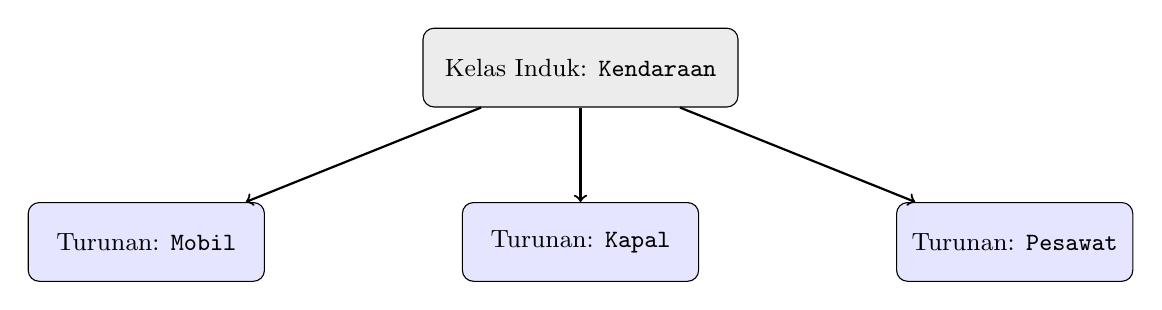
\begin{tikzpicture}[node distance=1.6cm, every node/.style={font=\small}]
\node (super) [draw, rectangle, rounded corners, fill=gray!15, 
minimum width=4cm, minimum height=1cm] 
{Kelas Induk: \texttt{Kendaraan}};
\node (mobil) [below left=1.2cm and 2.0cm of super, draw, rectangle, 
rounded corners, fill=blue!10, minimum width=3cm, minimum height=1cm] 
{Turunan: \texttt{Mobil}};
\node (kapal) [below=1.2cm of super, draw, rectangle, 
rounded corners, fill=blue!10, minimum width=3cm, minimum height=1cm] 
{Turunan: \texttt{Kapal}};
\node (pesawat) [below right=1.2cm and 2.0cm of super, draw, rectangle, 
rounded corners, fill=blue!10, minimum width=3cm, minimum height=1cm] 
{Turunan: \texttt{Pesawat}};
\draw[->, thick] (super) -- (mobil);
\draw[->, thick] (super) -- (kapal);
\draw[->, thick] (super) -- (pesawat);
\end{tikzpicture}
\end{center}

\subsection*{Ringkasan}
\begin{itemize}
    \item Polimorfisme: satu antarmuka, banyak bentuk perilaku.
    \item Dapat dicapai melalui pewarisan atau duck typing.
    \item Overriding memungkinkan perilaku disesuaikan oleh kelas turunan.
    \item Meningkatkan fleksibilitas, modularitas, dan keterbacaan kode.
\end{itemize}
\end{frame}

\section{Ringkasan}

\begin{frame}[fragile]{Rangkuman}
\vspace{20pt}
\begin{itemize}
    \item Bab ini membahas konsep dasar \textbf{OOP di Python}: kelas, objek, atribut, metode, pewarisan, dan polimorfisme.
    \item \textbf{Kelas} berfungsi sebagai cetak biru dari objek; \textbf{atribut} menyimpan keadaan; \textbf{metode} mendefinisikan perilaku.
    \item Penggunaan \texttt{super()} memungkinkan hierarki kelas yang efisien dan mencegah duplikasi kode.
    \item \textbf{Polimorfisme} memungkinkan objek berbeda merespons perintah yang sama dengan cara berbeda.
    \item Konsep \emph{duck typing} menambah fleksibilitas tanpa harus berbagi pewarisan langsung.
    \item Pemahaman konsep-konsep ini penting untuk membangun program yang \textbf{modular}, \textbf{reusable}, dan \textbf{mudah dirawat}.
\end{itemize}
\end{frame}



\end{document}